\documentclass[landscape]{article}

\usepackage[utf8]{inputenc}
\usepackage[english]{babel}

\usepackage{amsmath,amsfonts,amssymb}
\usepackage{fullpage}
\usepackage{verbatim}

\usepackage{tikz}
\usetikzlibrary{patterns}

% ------------------------------------------------------------------------------
% PgfPlots with TikZ

\usepackage{pgfplots}
\pgfplotsset{compat=1.12}

\usepgfplotslibrary{groupplots}

% space instead of thousand separator comma
\pgfkeys{/pgf/number format/.cd,1000 sep={\,}}

% another ylabel on the right:
\pgfplotsset{
    ylabel right/.style={
        after end axis/.append code={
            \node [rotate=270, anchor=south, yshift=3pt] at (rel axis cs:1,0.5) {#1};
        }
    }
}

\pgfplotsset{
    log x ticks with fixed point/.style={
        xticklabel={
            \pgfkeys{/pgf/fpu=true}
            \pgfmathparse{exp(\tick)}%
            \pgfmathprintnumber[fixed relative, precision=3]{\pgfmathresult}
            \pgfkeys{/pgf/fpu=false}
        }
    },
    log y ticks with fixed point/.style={
        yticklabel={
            \pgfkeys{/pgf/fpu=true}
            \pgfmathparse{exp(\tick)}%
            \pgfmathprintnumber[fixed relative, precision=3]{\pgfmathresult}
            \pgfkeys{/pgf/fpu=false}
        }
    }
}

\pgfplotsset{
    grid,
    major grid style={thin,dotted,color=black!50},
    minor grid style={thin,dotted,color=black!50},
    legend cell align=left,
    cycle list name={exotic},
    every axis/.append style={
        line width=0.5pt,
        tick style={
            line cap=round,
            thin,
            major tick length=4pt,
            minor tick length=2pt,
        },
    },
    legend style={
        /tikz/every even column/.append style={column sep=3mm,black},
        /tikz/every odd column/.append style={black},
    },
    % move title closer
    title style={yshift=-2pt},
    % less space on left and right
    enlarge x limits=0.04,
    every tick label/.append style={font=\small},
    %every axis label/.append style={font=\small},
    every axis y label/.append style={yshift=-1ex},
    xlabel near ticks,
    ylabel near ticks,
    legend columns=1,
    legend pos=north east,
}

\pgfplotsset{
    landscapePlot/.style={
        ybar,
        xtick=data,
        width=110mm,height=105mm,
        nodes near coords,
        nodes near coords align={vertical},
        enlarge y limits={upper,value=0.2},
        ymin=0,
        enlarge x limits=0.5,
    },
    batchTimePlot/.style={
        landscapePlot,
        title={Runtime},
        ylabel={SA construction time [s]},
        every axis y label/.style={at={(0,0.5)},xshift=-25pt,rotate=90},
    },
    batchMemPlot/.style={
        landscapePlot,
        title={Memory Utilization},
        ylabel={Extra Memory [MB]},
        every axis y label/.style={at={(0,0.5)},xshift=-34pt,rotate=90},
    },
}

%%%%%%%%%%%%%%%%%%%%%%%%%%%%%%%%%%%%%%%%%%%%%%%%%%%%%%%%%%%%%%%%%%%%%%%%%%%%%%%%

\begin{document}

\pgfplotscreateplotcyclelist{exotic}{%
    {fill=teal!50!white},
    {fill=orange!80!white},
    {fill=cyan!80!white},
    {fill=lime!80!white},
    {fill=red!80!white},
    {fill=yellow!80!white},
    {fill=black!60!white},
    {fill=blue!80!white},
    {fill=teal!80!white, postaction={pattern=north east lines}},
    {fill=orange!80!white, postaction={pattern=north east lines}},
    {fill=cyan!80!white, postaction={pattern=north east lines}},
    {fill=lime!80!white, postaction={pattern=north east lines}},
    {fill=red!80!white, postaction={pattern=north east lines}},
    {fill=yellow!80!white, postaction={pattern=north east lines}},
    {fill=black!80!white, postaction={pattern=north east lines}},
    {fill=blue!80!white, postaction={pattern=north east lines}},
    {fill=teal!80!white, postaction={pattern=north west lines}},
    {fill=orange!80!white, postaction={pattern=north west lines}},
    {fill=cyan!80!white, postaction={pattern=north west lines}},
    {fill=lime!80!white, postaction={pattern=north west lines}},
    {fill=red!80!white, postaction={pattern=north west lines}},
    {fill=yellow!80!white, postaction={pattern=north west lines}},
    {fill=black!80!white, postaction={pattern=north west lines}},
    {fill=blue!80!white, postaction={pattern=north west lines}},
    {fill=teal!80!white, postaction={pattern=dots}},
    {fill=orange!80!white, postaction={pattern=dots}},
    {fill=cyan!80!white, postaction={pattern=dots}},
    {fill=lime!80!white, postaction={pattern=dots}},
    {fill=red!80!white, postaction={pattern=dots}},
    {fill=yellow!80!white, postaction={pattern=dots}},
    {fill=black!80!white, postaction={pattern=dots}},
    {fill=blue!80!white, postaction={pattern=dots}},
    }

% IMPORT-DATA stats sqlplot.txt

\begin{figure}
    \centering\small

    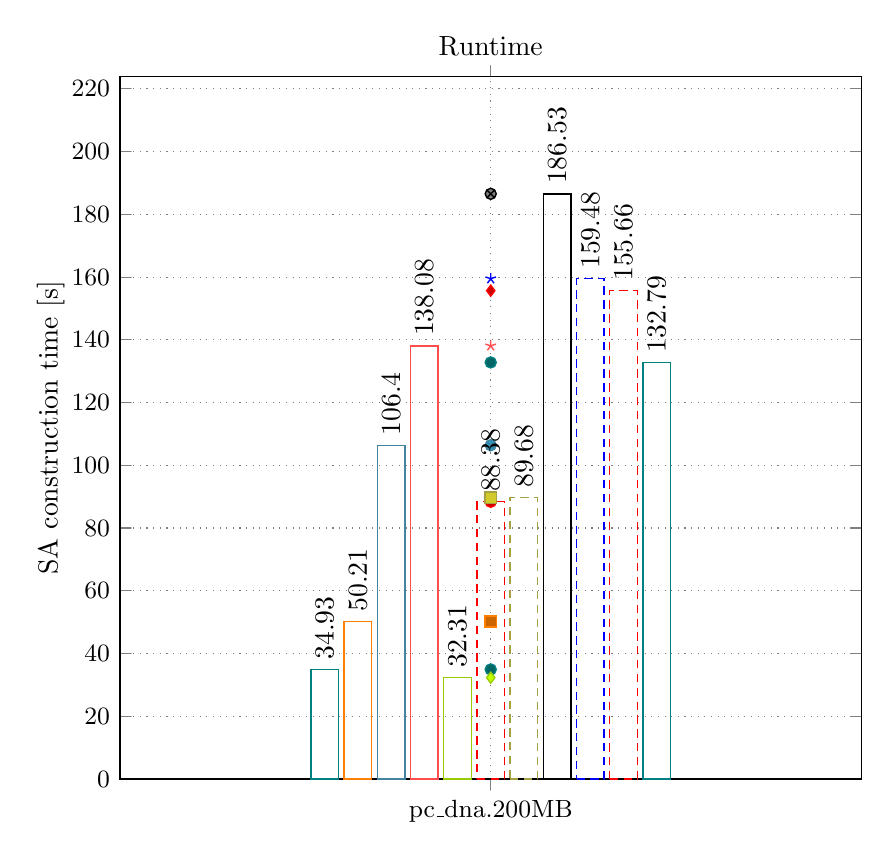
\begin{tikzpicture}
        \begin{axis}[batchTimePlot,
                cycle list name={exotic},
                legend to name=legend0,
                legend style={
                    /tikz/every even column/.append style={column sep=0.5cm,black},
                    /tikz/every even column/.append style={black},
                },
                legend columns=4,
                symbolic x coords={pc\_dna.200MB},
                every node near coord/.append style={color=black, rotate=90, anchor=west},
            ]

            %% MULTIPLOT(algo) SELECT algo, REPLACE(input, "_", "\_") AS x, time/1000 AS y
            %% FROM ( 
            %% SELECT algo, input, MEDIAN(memFinal) AS memFinal, MEDIAN(memOff) AS memOff, AVG(memPeak) AS memPeak, prefix, rep_i, threads, MEDIAN(time) AS time FROM stats GROUP BY algo, input, prefix, rep_i, threads
            %% ) WHERE input="pc_dna.200MB" AND threads=1 AND rep_i=0 GROUP BY MULTIPLOT,x ORDER BY algo
            \addplot coordinates { (pc\_dna.200MB,34.9312) };
            \addlegendentry{algo=BPR};
            \addplot coordinates { (pc\_dna.200MB,50.2121) };
            \addlegendentry{algo=BPR\_ref};
            \addplot coordinates { (pc\_dna.200MB,106.397) };
            \addlegendentry{algo=Deep-Shallow\_par};
            \addplot coordinates { (pc\_dna.200MB,138.08) };
            \addlegendentry{algo=Discarding4Parallel};
            \addplot coordinates { (pc\_dna.200MB,32.3096) };
            \addlegendentry{algo=DivSufSort\_ref};
            \addplot coordinates { (pc\_dna.200MB,88.3788) };
            \addlegendentry{algo=GSACA};
            \addplot coordinates { (pc\_dna.200MB,89.6768) };
            \addlegendentry{algo=GSACA\_parallel};
            \addplot coordinates { (pc\_dna.200MB,186.531) };
            \addlegendentry{algo=Osipov\_parallel};
            \addplot coordinates { (pc\_dna.200MB,159.483) };
            \addlegendentry{algo=Osipov\_parallel\_wp};
            \addplot coordinates { (pc\_dna.200MB,155.662) };
            \addlegendentry{algo=Osipov\_sequential};
            \addplot coordinates { (pc\_dna.200MB,132.79) };
            \addlegendentry{algo=Osipov\_sequential\_wp};
        \end{axis}
    \end{tikzpicture}
    \hfill
    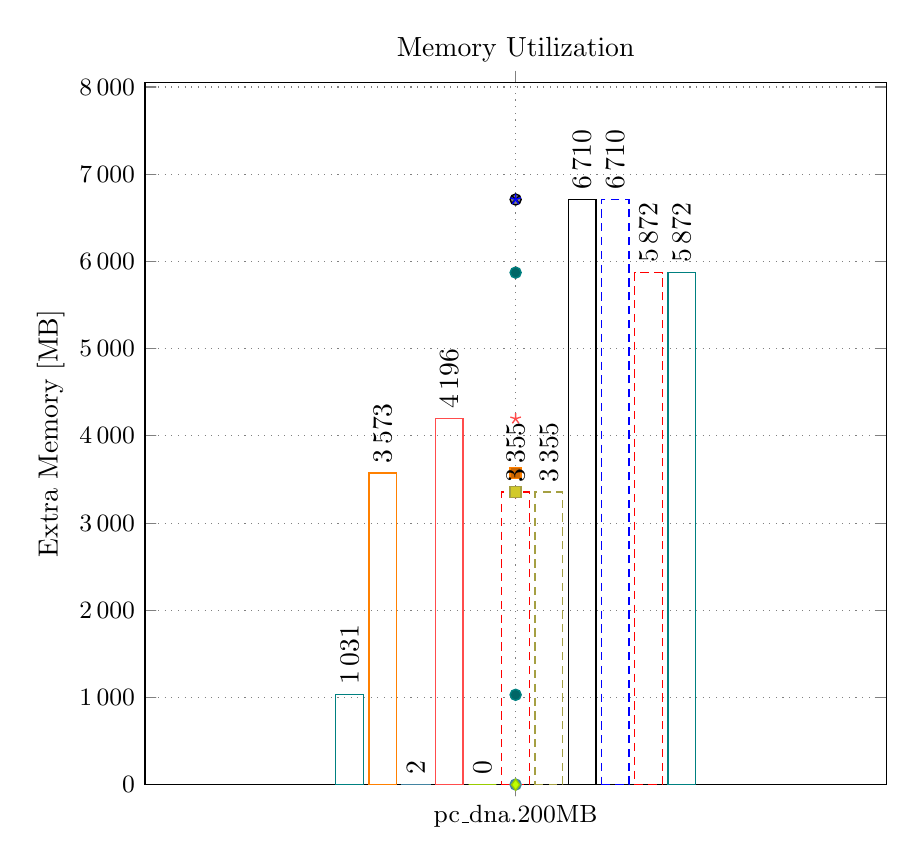
\begin{tikzpicture}
        \begin{axis}[batchMemPlot,
                symbolic x coords={pc\_dna.200MB},
                cycle list name={exotic},
                every node near coord/.append style={color=black, rotate=90, anchor=west},
            ]

            %% MULTIPLOT(algo) SELECT algo, REPLACE(input, "_", "\_") AS x, CEIL(memPeak/1000)/1000 AS y
            %% FROM ( 
            %% SELECT algo, input, MEDIAN(memFinal) AS memFinal, MEDIAN(memOff) AS memOff, AVG(memPeak) AS memPeak, prefix, rep_i, threads, MEDIAN(time) AS time FROM stats GROUP BY algo, input, prefix, rep_i, threads
            %% ) WHERE input="pc_dna.200MB" AND threads=1 AND rep_i=0 GROUP BY MULTIPLOT,x ORDER BY algo
            \addplot coordinates { (pc\_dna.200MB,1031) };
            \addlegendentry{algo=BPR};
            \addplot coordinates { (pc\_dna.200MB,3573) };
            \addlegendentry{algo=BPR\_ref};
            \addplot coordinates { (pc\_dna.200MB,2) };
            \addlegendentry{algo=Deep-Shallow\_par};
            \addplot coordinates { (pc\_dna.200MB,4196) };
            \addlegendentry{algo=Discarding4Parallel};
            \addplot coordinates { (pc\_dna.200MB,0) };
            \addlegendentry{algo=DivSufSort\_ref};
            \addplot coordinates { (pc\_dna.200MB,3355) };
            \addlegendentry{algo=GSACA};
            \addplot coordinates { (pc\_dna.200MB,3355) };
            \addlegendentry{algo=GSACA\_parallel};
            \addplot coordinates { (pc\_dna.200MB,6710) };
            \addlegendentry{algo=Osipov\_parallel};
            \addplot coordinates { (pc\_dna.200MB,6710) };
            \addlegendentry{algo=Osipov\_parallel\_wp};
            \addplot coordinates { (pc\_dna.200MB,5872) };
            \addlegendentry{algo=Osipov\_sequential};
            \addplot coordinates { (pc\_dna.200MB,5872) };
            \addlegendentry{algo=Osipov\_sequential\_wp};

            \legend{}
        \end{axis}
    \end{tikzpicture}

    \medskip
    \ref{legend0}
\end{figure}

\begin{figure}
    \centering\small

    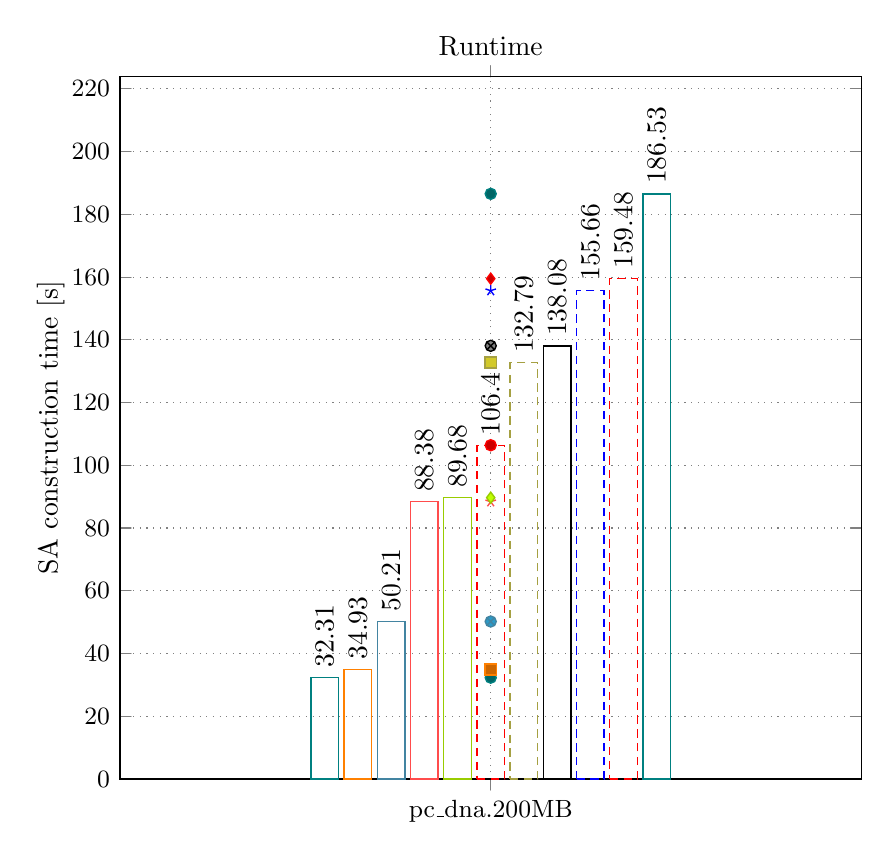
\begin{tikzpicture}
        \begin{axis}[batchTimePlot,
                cycle list name={exotic},
                legend to name=legend1,
                legend style={
                    /tikz/every even column/.append style={column sep=0.5cm,black},
                    /tikz/every even column/.append style={black},
                },
                legend columns=4,
                symbolic x coords={pc\_dna.200MB},
                every node near coord/.append style={color=black, rotate=90, anchor=west},
            ]

            %% MULTIPLOT(algo) SELECT algo, REPLACE(input, "_", "\_") AS x, time/1000 AS y
            %% FROM ( 
            %% SELECT algo, input, MEDIAN(memFinal) AS memFinal, MEDIAN(memOff) AS memOff, AVG(memPeak) AS memPeak, prefix, rep_i, threads, MEDIAN(time) AS time FROM stats GROUP BY algo, input, prefix, rep_i, threads
            %% ) WHERE input="pc_dna.200MB" AND threads=1 AND rep_i=0 GROUP BY MULTIPLOT,x ORDER BY time
            \addplot coordinates { (pc\_dna.200MB,32.3096) };
            \addlegendentry{algo=DivSufSort\_ref};
            \addplot coordinates { (pc\_dna.200MB,34.9312) };
            \addlegendentry{algo=BPR};
            \addplot coordinates { (pc\_dna.200MB,50.2121) };
            \addlegendentry{algo=BPR\_ref};
            \addplot coordinates { (pc\_dna.200MB,88.3788) };
            \addlegendentry{algo=GSACA};
            \addplot coordinates { (pc\_dna.200MB,89.6768) };
            \addlegendentry{algo=GSACA\_parallel};
            \addplot coordinates { (pc\_dna.200MB,106.397) };
            \addlegendentry{algo=Deep-Shallow\_par};
            \addplot coordinates { (pc\_dna.200MB,132.79) };
            \addlegendentry{algo=Osipov\_sequential\_wp};
            \addplot coordinates { (pc\_dna.200MB,138.08) };
            \addlegendentry{algo=Discarding4Parallel};
            \addplot coordinates { (pc\_dna.200MB,155.662) };
            \addlegendentry{algo=Osipov\_sequential};
            \addplot coordinates { (pc\_dna.200MB,159.483) };
            \addlegendentry{algo=Osipov\_parallel\_wp};
            \addplot coordinates { (pc\_dna.200MB,186.531) };
            \addlegendentry{algo=Osipov\_parallel};
        \end{axis}
    \end{tikzpicture}
    \hfill
    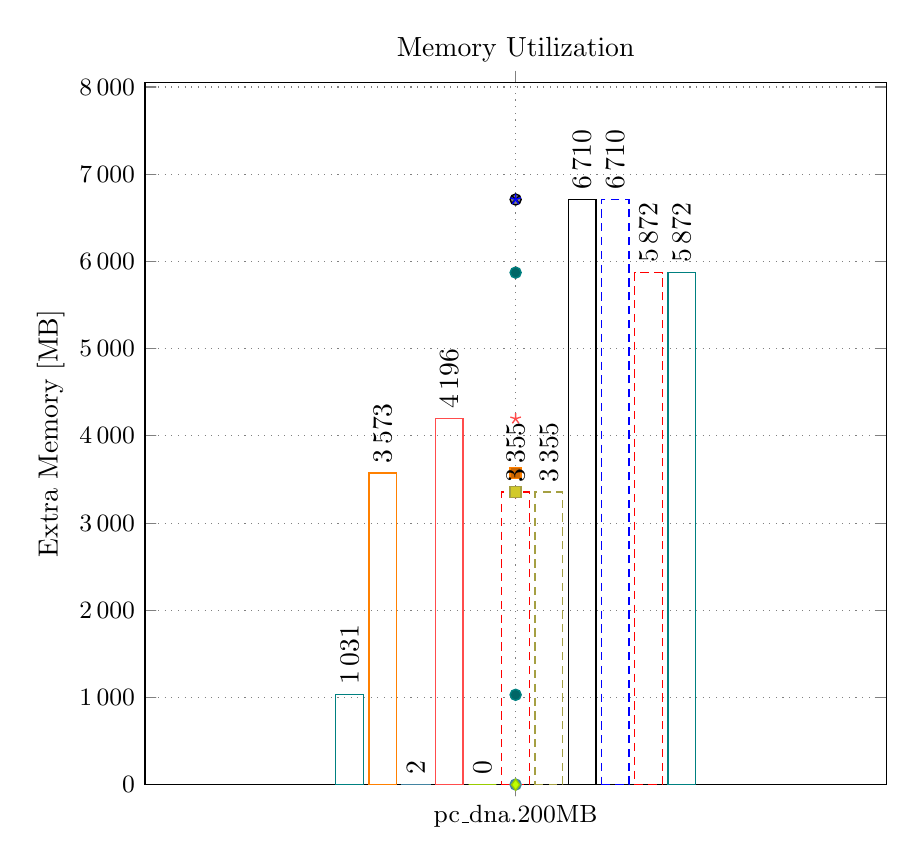
\begin{tikzpicture}
        \begin{axis}[batchMemPlot,
                symbolic x coords={pc\_dna.200MB},
                cycle list name={exotic},
                every node near coord/.append style={color=black, rotate=90, anchor=west},
            ]

            %% MULTIPLOT(algo) SELECT algo, REPLACE(input, "_", "\_") AS x, CEIL(memPeak/1000)/1000 AS y
            %% FROM ( 
            %% SELECT algo, input, MEDIAN(memFinal) AS memFinal, MEDIAN(memOff) AS memOff, AVG(memPeak) AS memPeak, prefix, rep_i, threads, MEDIAN(time) AS time FROM stats GROUP BY algo, input, prefix, rep_i, threads
            %% ) WHERE input="pc_dna.200MB" AND threads=1 AND rep_i=0 GROUP BY MULTIPLOT,x ORDER BY algo
            \addplot coordinates { (pc\_dna.200MB,1031) };
            \addlegendentry{algo=BPR};
            \addplot coordinates { (pc\_dna.200MB,3573) };
            \addlegendentry{algo=BPR\_ref};
            \addplot coordinates { (pc\_dna.200MB,2) };
            \addlegendentry{algo=Deep-Shallow\_par};
            \addplot coordinates { (pc\_dna.200MB,4196) };
            \addlegendentry{algo=Discarding4Parallel};
            \addplot coordinates { (pc\_dna.200MB,0) };
            \addlegendentry{algo=DivSufSort\_ref};
            \addplot coordinates { (pc\_dna.200MB,3355) };
            \addlegendentry{algo=GSACA};
            \addplot coordinates { (pc\_dna.200MB,3355) };
            \addlegendentry{algo=GSACA\_parallel};
            \addplot coordinates { (pc\_dna.200MB,6710) };
            \addlegendentry{algo=Osipov\_parallel};
            \addplot coordinates { (pc\_dna.200MB,6710) };
            \addlegendentry{algo=Osipov\_parallel\_wp};
            \addplot coordinates { (pc\_dna.200MB,5872) };
            \addlegendentry{algo=Osipov\_sequential};
            \addplot coordinates { (pc\_dna.200MB,5872) };
            \addlegendentry{algo=Osipov\_sequential\_wp};

            \legend{}
        \end{axis}
    \end{tikzpicture}

    \medskip
    \ref{legend1}
\end{figure}

\begin{figure}
    \centering\small

    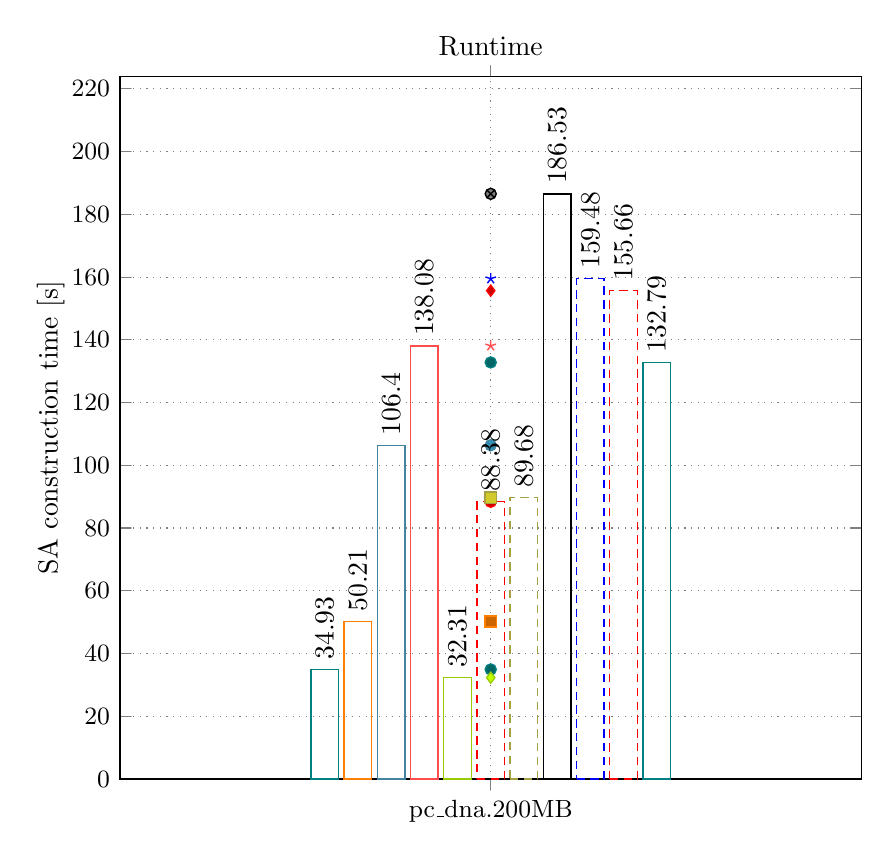
\begin{tikzpicture}
        \begin{axis}[batchTimePlot,
                cycle list name={exotic},
                legend to name=legend2,
                legend style={
                    /tikz/every even column/.append style={column sep=0.5cm,black},
                    /tikz/every even column/.append style={black},
                },
                legend columns=4,
                symbolic x coords={pc\_dna.200MB},
                every node near coord/.append style={color=black, rotate=90, anchor=west},
            ]

            %% MULTIPLOT(algo) SELECT algo, REPLACE(input, "_", "\_") AS x, time/1000 AS y
            %% FROM ( 
            %% SELECT algo, input, MEDIAN(memFinal) AS memFinal, MEDIAN(memOff) AS memOff, AVG(memPeak) AS memPeak, prefix, rep_i, threads, MEDIAN(time) AS time FROM stats GROUP BY algo, input, prefix, rep_i, threads
            %% ) WHERE input="pc_dna.200MB" AND threads=1 AND rep_i=0 GROUP BY MULTIPLOT,x ORDER BY algo
            \addplot coordinates { (pc\_dna.200MB,34.9312) };
            \addlegendentry{algo=BPR};
            \addplot coordinates { (pc\_dna.200MB,50.2121) };
            \addlegendentry{algo=BPR\_ref};
            \addplot coordinates { (pc\_dna.200MB,106.397) };
            \addlegendentry{algo=Deep-Shallow\_par};
            \addplot coordinates { (pc\_dna.200MB,138.08) };
            \addlegendentry{algo=Discarding4Parallel};
            \addplot coordinates { (pc\_dna.200MB,32.3096) };
            \addlegendentry{algo=DivSufSort\_ref};
            \addplot coordinates { (pc\_dna.200MB,88.3788) };
            \addlegendentry{algo=GSACA};
            \addplot coordinates { (pc\_dna.200MB,89.6768) };
            \addlegendentry{algo=GSACA\_parallel};
            \addplot coordinates { (pc\_dna.200MB,186.531) };
            \addlegendentry{algo=Osipov\_parallel};
            \addplot coordinates { (pc\_dna.200MB,159.483) };
            \addlegendentry{algo=Osipov\_parallel\_wp};
            \addplot coordinates { (pc\_dna.200MB,155.662) };
            \addlegendentry{algo=Osipov\_sequential};
            \addplot coordinates { (pc\_dna.200MB,132.79) };
            \addlegendentry{algo=Osipov\_sequential\_wp};
        \end{axis}
    \end{tikzpicture}
    \hfill
    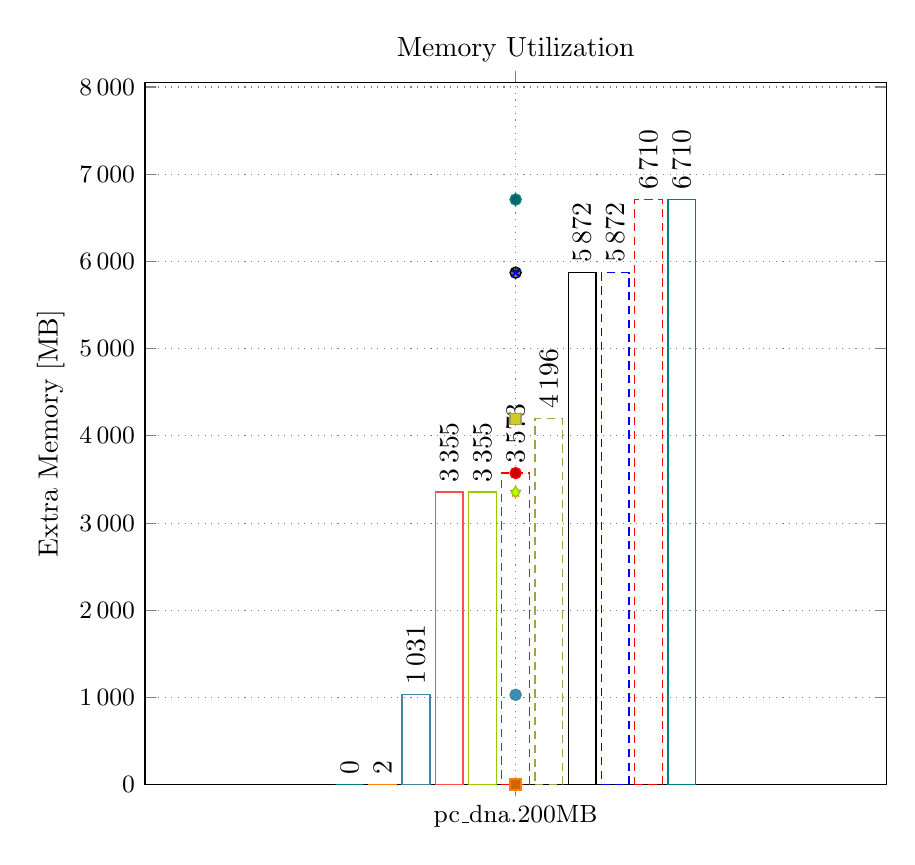
\begin{tikzpicture}
        \begin{axis}[batchMemPlot,
                symbolic x coords={pc\_dna.200MB},
                cycle list name={exotic},
                every node near coord/.append style={color=black, rotate=90, anchor=west},
            ]

            %% MULTIPLOT(algo) SELECT algo, REPLACE(input, "_", "\_") AS x, CEIL(memPeak/1000)/1000 AS y
            %% FROM ( 
            %% SELECT algo, input, MEDIAN(memFinal) AS memFinal, MEDIAN(memOff) AS memOff, AVG(memPeak) AS memPeak, prefix, rep_i, threads, MEDIAN(time) AS time FROM stats GROUP BY algo, input, prefix, rep_i, threads
            %% ) WHERE input="pc_dna.200MB" AND threads=1 AND rep_i=0 GROUP BY MULTIPLOT,x ORDER BY memPeak
            \addplot coordinates { (pc\_dna.200MB,0) };
            \addlegendentry{algo=DivSufSort\_ref};
            \addplot coordinates { (pc\_dna.200MB,2) };
            \addlegendentry{algo=Deep-Shallow\_par};
            \addplot coordinates { (pc\_dna.200MB,1031) };
            \addlegendentry{algo=BPR};
            \addplot coordinates { (pc\_dna.200MB,3355) };
            \addlegendentry{algo=GSACA};
            \addplot coordinates { (pc\_dna.200MB,3355) };
            \addlegendentry{algo=GSACA\_parallel};
            \addplot coordinates { (pc\_dna.200MB,3573) };
            \addlegendentry{algo=BPR\_ref};
            \addplot coordinates { (pc\_dna.200MB,4196) };
            \addlegendentry{algo=Discarding4Parallel};
            \addplot coordinates { (pc\_dna.200MB,5872) };
            \addlegendentry{algo=Osipov\_sequential};
            \addplot coordinates { (pc\_dna.200MB,5872) };
            \addlegendentry{algo=Osipov\_sequential\_wp};
            \addplot coordinates { (pc\_dna.200MB,6710) };
            \addlegendentry{algo=Osipov\_parallel};
            \addplot coordinates { (pc\_dna.200MB,6710) };
            \addlegendentry{algo=Osipov\_parallel\_wp};

            \legend{}
        \end{axis}
    \end{tikzpicture}

    \medskip
    \ref{legend2}
\end{figure}

\end{document}

